\paragraph{Protéine choisie.} Nous avons choisi la \textbf{calmoduline-1 humaine} (\emph{Homo sapiens}, gène \emph{CALM1}), identifiant UniProtKB \textbf{P0DP23}~\cite{uniprot_P0DP23,uniprot2023}, de \textbf{149 résidus}. Voici la séquence utilisée, telle que fournie par UniProt (fichier \texttt{data/P0DP23.fasta}) :

\begin{center}
\scriptsize\ttfamily
MADQLTEEQIAEFKEAFSLFDKDGDGTITTKELGTVMRSLGQNPTEAELQDMINEVDADG\\
NGTIDFPEFLTMMARKMKDTDSEEEIREAFRVFDKDGNGYISAAELRHVMTNLGEKLTDE\\
EVDEMIREADIDGDGQVNYEEFVQMMTAK
\end{center}

Ce choix a trois raisons. D'abord, la taille est compatible avec un calcul sur CPU. Ensuite, la protéine est très étudiée et sa structure expérimentale est connue (par exemple PDB 1CLL~\cite{chattopadhyaya1992}). Enfin, et surtout, sa structure en \og haltère \fg{} se prête bien à l'analyse des scores de confiance : deux lobes globulaires (chacun formé de deux motifs EF-hand fixant le Ca$^{2+}$) sont reliés par une région centrale connue pour être flexible en solution~\cite{barbato1992}. On s'attend donc à ce que le pLDDT et la PAE ne racontent pas la même chose.

\paragraph{Exécution.} La commande \texttt{colabfold\_batch --num-models 5} a été lancée avec les paramètres par défaut : MSA \texttt{mmseqs2\_uniref\_env}, pas de gabarits, pas de relaxation Amber, 3 recyclages. Le MSA, construit en environ 15~s, contient \textbf{21\,884 séquences}. Chacun des 5 modèles a demandé environ 23~min sur CPU, soit \textbf{1~h~57 au total}. Le tableau~\ref{tab:fichiers} présente les fichiers importants produits dans \texttt{results/P0DP23/}.

\begin{table}[H]
\centering
\footnotesize
\begin{tabularx}{\textwidth}{>{\ttfamily\raggedright\arraybackslash}p{6.2cm}X}
\toprule
\normalfont\textbf{Fichier} & \textbf{Contenu} \\
\midrule
*\_unrelaxed\_rank\_001\_*.pdb & \textbf{Structure prédite} (format PDB) du meilleur modèle ; le pLDDT est stocké dans la colonne \emph{B-factor} \\
*\_scores\_rank\_001\_*.json & Clés \texttt{plddt} (149 valeurs), \texttt{pae} (matrice 149$\times$149 en Å), \texttt{ptm} \\
*\_rank\_002 \ldots 005\_* & Les 4 autres modèles, classés par pLDDT moyen décroissant \\
*.a3m, *\_coverage.png & MSA utilisé et profondeur de l'alignement par position \\
log.txt, config.json & Journal et paramètres exacts, pour la traçabilité \\
\bottomrule
\end{tabularx}
\caption{Principaux fichiers produits par ColabFold.}
\label{tab:fichiers}
\end{table}

\paragraph{Structure obtenue.} Le meilleur modèle (modèle~4) a un pLDDT moyen de 82,8 et un pTM de 0,487. Les 5 modèles sont très proches : pLDDT moyens entre 78,6 et 82,8, pTM entre 0,458 et 0,487. La structure (figure~\ref{fig:structure}) présente bien deux lobes compacts d'hélices $\alpha$, dont les centres sont distants de 32,6~Å, reliés par une région centrale étirée.

\begin{figure}[H]
  \centering
  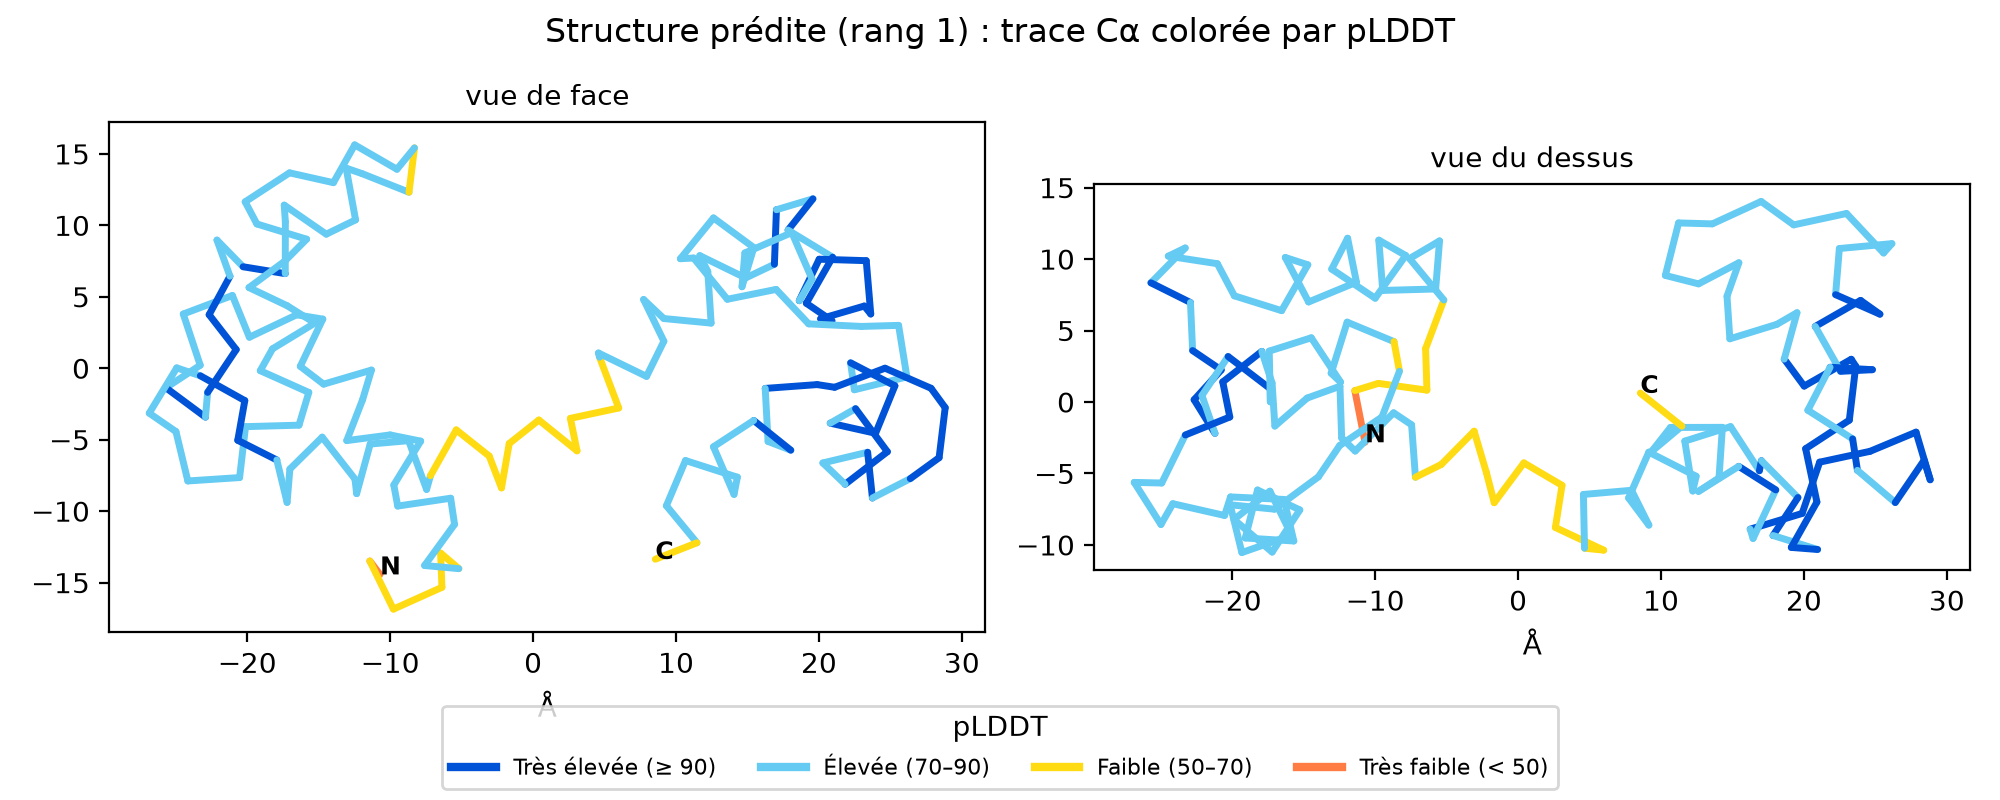
\includegraphics[width=0.95\textwidth]{../figures/P0DP23/structure.png}
  \caption{Trace C$\alpha$ du meilleur modèle, colorée par pLDDT (produite par \texttt{scripts/analyse.py}). Elle peut aussi être visualisée en 3D en déposant le fichier PDB sur \url{https://molstar.org/viewer/}.}
  \label{fig:structure}
\end{figure}

%====================================================================
\section{Analyse des scores de confiance}
\label{sec:analyse}
%====================================================================

Les deux scores se trouvent dans le fichier \texttt{*\_scores\_rank\_001\_*.json}. Le script \texttt{scripts/analyse.py} le lit avec le module \texttt{json} de Python et produit les figures ainsi qu'un résumé chiffré (\texttt{figures/P0DP23/resume.txt}). Il vérifie aussi que le pLDDT lu dans le JSON est identique à celui stocké dans la colonne B-factor du PDB (écart maximal : 0,00).

\subsection{pLDDT : confiance locale}

\paragraph{Définition.} Le pLDDT (\emph{predicted Local Distance Difference Test}) est une note de 0 à 100 attribuée à \emph{chaque résidu}. Il estime le score lDDT-C$\alpha$~\cite{mariani2013} que la prédiction obtiendrait si on la comparait à la vraie structure. Autrement dit, il indique si les distances entre ce résidu et ses voisins proches sont correctes. Ce score est \emph{local} et ne nécessite aucune superposition~\cite{jumper2021,ebi_course}.
\begin{itemize}
  \item \textbf{$>$ 90} : très fiable, squelette et chaînes latérales compris ;
  \item \textbf{70–90} : squelette fiable, chaînes latérales parfois mal placées ;
  \item \textbf{50–70} : faible confiance ;
  \item \textbf{$<$ 50} : à ne pas interpréter. C'est souvent une région intrinsèquement désordonnée, mais cela peut aussi signifier que l'information manque, par exemple un linker entre deux domaines.
\end{itemize}
Le pLDDT sert donc à décider quelles parties de la structure on peut exploiter. En revanche, un pLDDT élevé partout \emph{ne garantit pas} que les domaines sont correctement placés les uns par rapport aux autres~\cite{ebi_course}.

\begin{figure}[H]
  \centering
  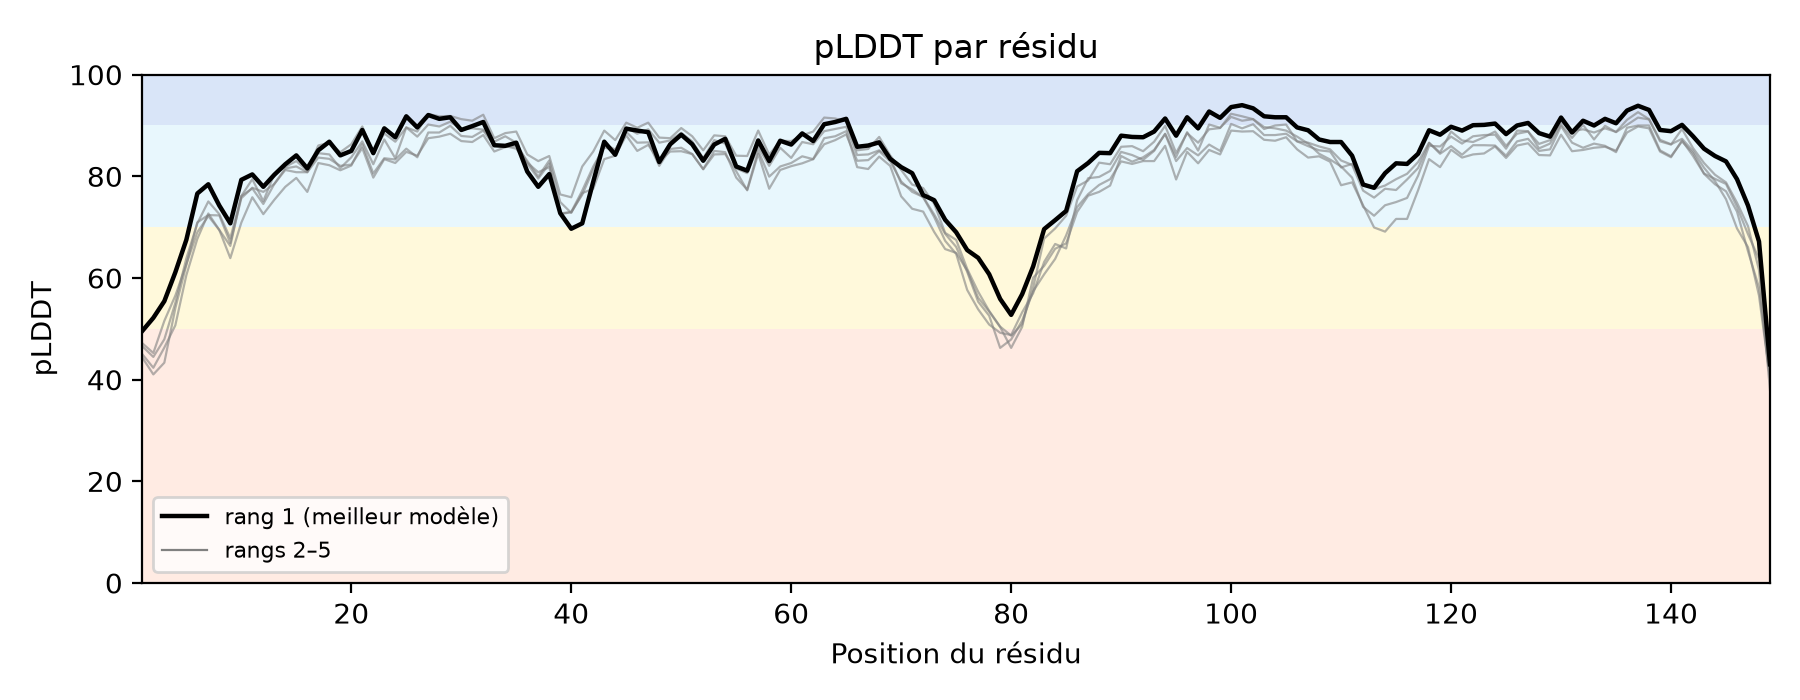
\includegraphics[width=0.95\textwidth]{../figures/P0DP23/plddt.png}
  \caption{pLDDT par résidu du meilleur modèle (noir) et des 4 autres (gris). Fonds colorés : classes de confiance.}
  \label{fig:plddt}
\end{figure}

\paragraph{Résultats.} La figure~\ref{fig:plddt} montre que 88,6~\% des résidus ont un pLDDT supérieur à 70 : 21,5~\% au-dessus de 90 et 67,1~\% entre 70 et 90. Les deux lobes (environ 6–72 et 86–145) sont prédits avec confiance, avec des maxima au-dessus de 90 dans les hélices. Trois zones descendent sous 70 :
\begin{itemize}
  \item \textbf{la région centrale 75–83} (minimum de 53 au résidu 80) : c'est le linker entre les deux lobes, dont la flexibilité en solution est connue~\cite{barbato1992} ;
  \item \textbf{les extrémités 1–5 et 148–149} (minimum de 43 au résidu C-terminal) : les extrémités libres d'une chaîne sont typiquement peu contraintes ;
  \item un léger creux vers le résidu 40, et un autre autour de 112–113 (environ 78), à la jonction entre les deux motifs EF-hand de chaque lobe.
\end{itemize}
Les 5 modèles donnent le même profil (courbes grises), ce qui montre que ces variations ne sont pas dues au hasard d'un seul modèle.

\subsection{PAE : confiance dans les positions relatives}

\paragraph{Définition.} La PAE (\emph{Predicted Aligned Error}) est une \emph{matrice} N$\times$N. La valeur (i,j) est l'erreur attendue, en ångströms, sur la position du résidu~\emph{i} si l'on superpose la prédiction et la vraie structure sur le résidu~\emph{j}~\cite{ebi_course}. Les deux axes représentent donc les résidus de la protéine : en ordonnée, le résidu dont on évalue la position ; en abscisse, le résidu sur lequel on aligne. La diagonale, qui correspond à l'alignement d'un résidu sur lui-même, vaut toujours presque zéro et ne porte pas d'information. Une valeur faible (vert foncé) signifie que la position relative des deux résidus est fiable ; une valeur élevée (vert clair) signifie qu'elle ne l'est pas.

\paragraph{Différence avec le pLDDT.} Le pLDDT répond à la question \og ce résidu est-il bien placé par rapport à ses voisins ? \fg{} ; la PAE répond à la question \og la position de ce résidu \emph{par rapport à ce résidu éloigné} est-elle fiable ? \fg{}. La PAE est donc indispensable pour juger l'\textbf{arrangement des domaines}.

\begin{figure}[H]
  \centering
  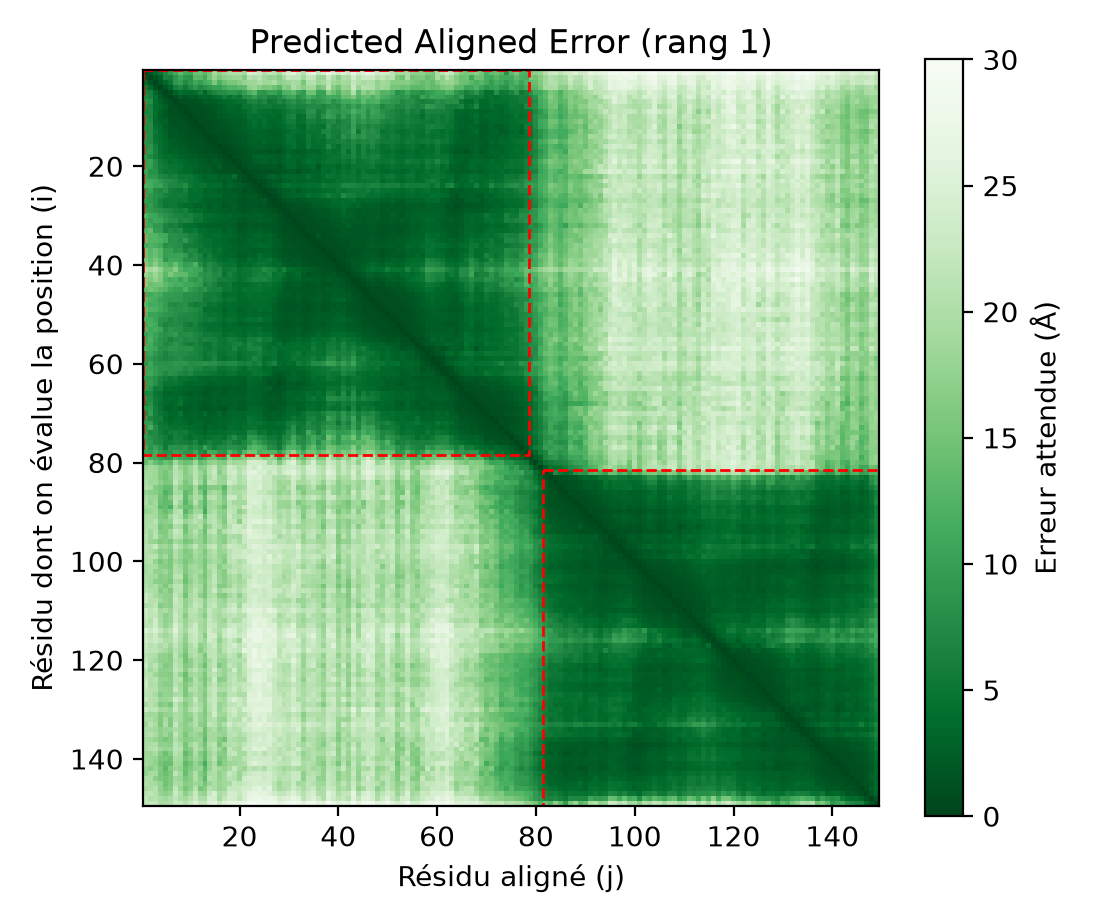
\includegraphics[width=0.55\textwidth]{../figures/P0DP23/pae.png}
  \caption{Matrice PAE du meilleur modèle. Cadres rouges : lobe N (1–78) et lobe C (82–149).}
  \label{fig:pae}
\end{figure}

\paragraph{Résultats.} La matrice (figure~\ref{fig:pae}) montre \textbf{deux blocs vert foncé} le long de la diagonale, qui correspondent aux deux lobes. La PAE moyenne vaut 5,1~Å à l'intérieur du lobe N et 3,8~Å à l'intérieur du lobe C : chaque lobe est une unité rigide bien prédite. En revanche, les \textbf{blocs hors diagonale} sont clairs, avec une PAE moyenne de 20,6 et 19,7~Å entre les deux lobes. AlphaFold2 est donc sûr de la forme de chaque lobe, mais \emph{pas} de leur orientation l'une par rapport à l'autre.

C'est l'exemple typique où le pLDDT seul induirait en erreur. Hormis le linker, presque tous les résidus ont un pLDDT supérieur à 70, et pourtant la position relative des lobes dans le fichier PDB n'est qu'une conformation parmi d'autres possibles. Ce résultat est cohérent avec le pTM modeste (0,49) et avec la flexibilité connue de la calmoduline, dont la région centrale se replie pour envelopper ses peptides cibles. Enfin, AlphaFold2 ignore les ions : la structure est prédite sans les quatre Ca$^{2+}$ qui, dans la cellule, modifient la conformation des lobes.
